\begin{figure*}[t]
  \centering
  \begin{subfigure}[t]{0.32\textwidth}
    \centering
    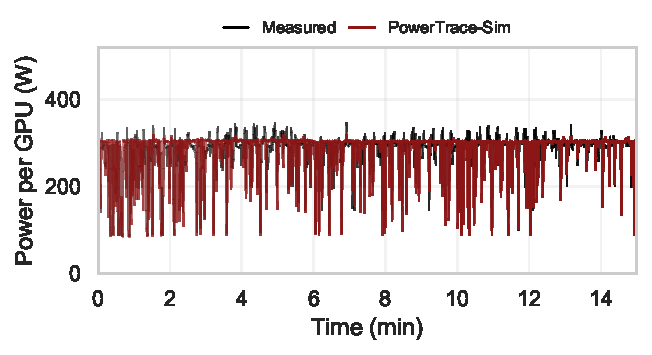
\includegraphics[width=\linewidth]{results/paper/appendix/power_trace_burstgpt_qwen3_8b_a100_tp1_stratum_0_idle_1s.pdf}
    \caption{Fano stratum 0 (851 requests).
    Replacing only the source idle floor
    (70.1~W/GPU) with the run's declared
    pre-request idle (85.0~W/GPU) changes energy
    error from 3.82\% to
    1.60\%, with 0.099
    NRMSE, 0.0085 Soft-DTW, and ACF
    $R^2=0.347$.}
    \label{fig:burstgpt-stratum-0}
  \end{subfigure}\hfill
  \begin{subfigure}[t]{0.32\textwidth}
    \centering
    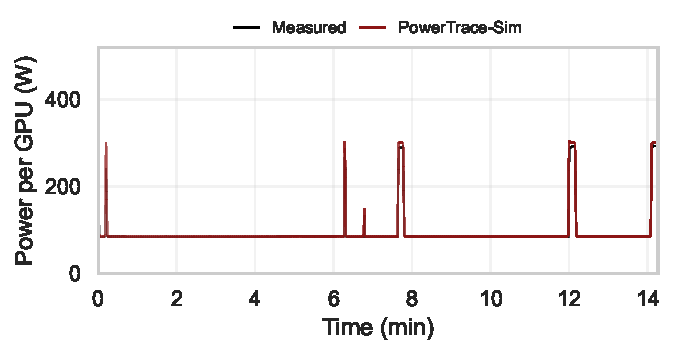
\includegraphics[width=\linewidth]{results/paper/appendix/power_trace_burstgpt_qwen3_8b_a100_tp1_stratum_1_idle_1s.pdf}
    \caption{Fano stratum 1 (7 requests).
    Replacing only the source idle floor
    (70.1~W/GPU) with the run's declared
    pre-request idle (85.4~W/GPU) changes energy
    error from 15.27\% to
    1.16\%, with 0.029
    NRMSE, 0.0009 Soft-DTW, and ACF
    $R^2=0.999$.}
    \label{fig:burstgpt-stratum-1}
  \end{subfigure}\hfill
  \begin{subfigure}[t]{0.32\textwidth}
    \centering
    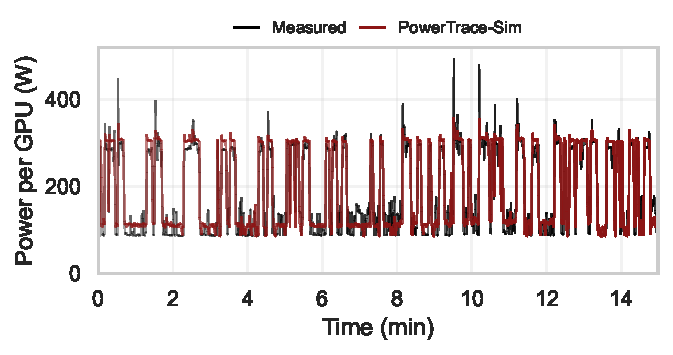
\includegraphics[width=\linewidth]{results/paper/appendix/power_trace_burstgpt_qwen3_8b_a100_tp1_stratum_2_idle_1s.pdf}
    \caption{Fano stratum 2 (1,755 requests).
    Replacing only the source idle floor
    (70.1~W/GPU) with the run's declared
    pre-request idle (85.1~W/GPU) changes energy
    error from 4.77\% to
    3.25\%, with 0.068
    NRMSE, 0.0042 Soft-DTW, and ACF
    $R^2=0.994$.}
    \label{fig:burstgpt-stratum-2}
  \end{subfigure}
  \caption{Transfer to exact BurstGPT arbitrary-arrival replays on Qwen3-8B
  A100 TP1. Black is measured power and red is PowerTrace-Sim from the exact
  replay marks; both are matched one-second per-GPU means over the complete
  common interval. The timing and dynamic power laws remain frozen, and each
  panel changes only its separately measured 60-second pre-request idle
  intercept. Across all three disjoint strata, idle-calibrated energy error is
  1.16--3.25\%, range NRMSE is at most
  0.099, and Soft-DTW is at most 0.0085.
  ACF agreement is strong for strata 1--2 but only moderate for stratum 0, where
  the model underestimates the largest power pulses. Because the idle rule was
  applied after these sealed targets were inspected, this is retrospective
  arbitrary-arrival evidence rather than a sealed zero-shot claim.}
  \label{fig:burstgpt-idle-transfer}
\end{figure*}
